\documentclass[12pt, english]{report_template}
\usepackage{amsmath}
\usepackage{graphicx}
\usepackage{subcaption} % For subfigures
\usepackage{pythonhighlight} % For python code highlighting
\usepackage{lipsum}
\usepackage[hidelinks]{hyperref}

% Packages for pseudo-code environment and algorithm environment
\usepackage{pseudo}
\usepackage{tcolorbox}
\usepackage{tabto}
\tcbuselibrary{skins,theorems}
\TabPositions{1.5cm}
\newtcbtheorem{algorithm}{Algorithm}{pseudo/ruled, float}{alg}

\graphicspath{{figures/}}

% Define document
\title{TSFS12 Hand-in 1: \\
Discrete Path Planning in a Structured Road Network}
\author[email=first.last@student.liu.se, liuid=firla123]{Firstname Lastname}
\author[email=first.last@student.liu.se, liuid=firla123]{Firstname Lastname}
\date{\today}

\addbibresource{references.bib}

\begin{document}
\maketitle

\section{Introduction}
\label{sec:introduction}

Some references: Section~\ref{sec:introduction}, Section~\ref{sec:introduction_sub}, \eqref{eq:abc}, Figure~\ref{fig:blue_marble}, and Table~\ref{tab:example_table}.
Algorithm~\ref{alg:euclid}.

\cite{lavalle2006planning, dubins1957curves, karaman2011sampling, limebeer2015faster, paden2016survey, rawlings2020model} and \cite{oh2015survey}.

Equations can be included
\begin{equation}
	\label{eq:abc}
	f(t + h) = f(t) + f'(t)  h + \frac{1}{2!}f''(t)  h^2 + \mathcal{O}(h^3)
\end{equation}
Remember to use scalable vector graphics (PDF) for plots and figures, bitmaps is for photos.
\begin{figure}
	\centering
	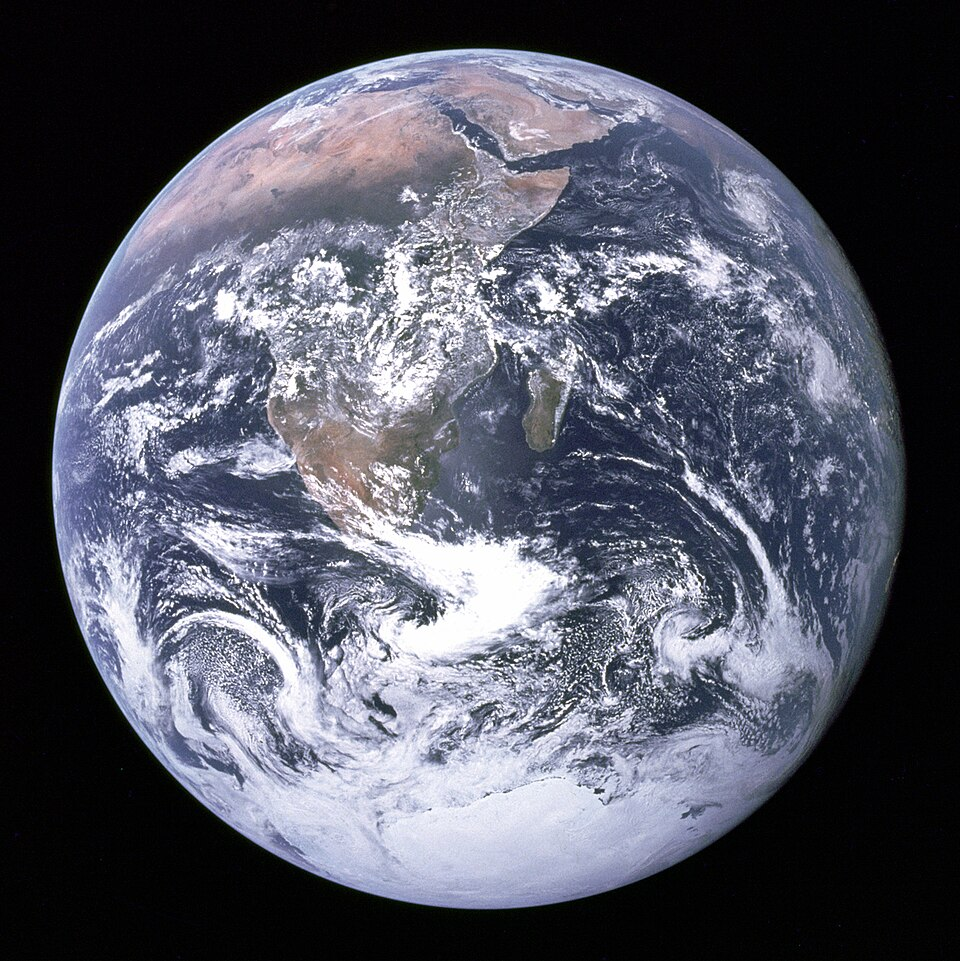
\includegraphics[width=0.4\textwidth]{blue_marble.jpg}
	\caption{The famous blue marble photo (\url{https://en.wikipedia.org/wiki/The_Blue_Marble}).}
	\label{fig:blue_marble}
\end{figure}
Tables can also be included, as in \ref{tab:example_table}.
\begin{table}
	\centering
	\caption{An example table.}
	\label{tab:example_table}
	\begin{tabular}{cc}
		\textbf{Column One} & \textbf{Column Two} \\
		\hline
		One                 & Two                 \\
		Three               & Four
	\end{tabular}
\end{table}

Code can be directly included in the text, e.g., using the \texttt{pythonhighlight} package.
\begin{python}
    def gcd(a, b):
    "Compute the GCD of a and b using Euclid's algorithm."
    while b:
        a, b = b, a % b
    return a
\end{python}
\lipsum[1-2]
\begin{algorithm}{Euclid's algorithm, \pr{Euclid}(a, b)}{}
	\label{alg:euclid}
	\textbf{Input:} Two positive integers, $a$ and $b$.\\
	\textbf{Output:} The greatest common divisor of $a$ and $b$.

	\begin{pseudo}[label=\small\arabic*, indent-mark, ]
\textbf{while} $a \neq b$\\+
    \textbf{if} $a > b$ \\+
        $a = a - b$\\-
    \textbf{else} $b = b - a$\\-
\textbf{return} $a$
\end{pseudo}
	The running time is quadratic in the number of bits in the input.
\end{algorithm}

\subsection{Introduction}
\label{sec:introduction_sub}

\lipsum[1]

\begin{figure}
	\centering
	\subcaptionbox{}{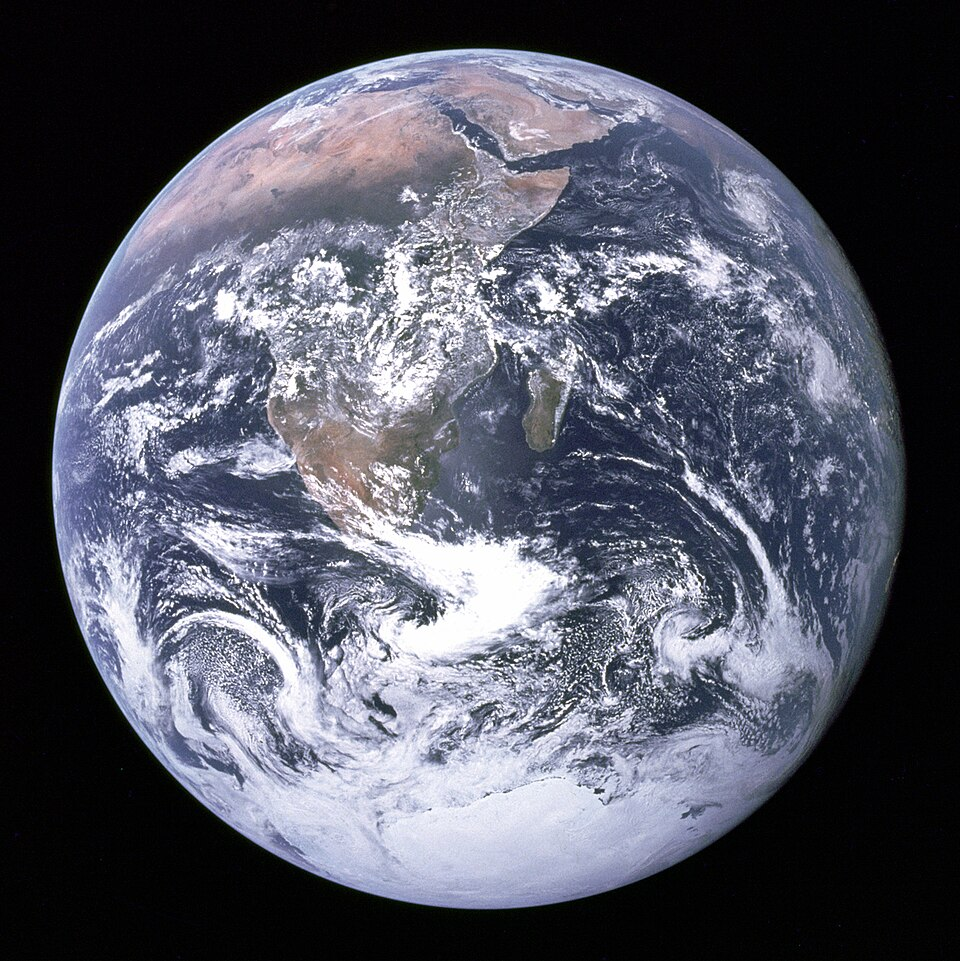
\includegraphics[width=50mm]{blue_marble.jpg}}
	\subcaptionbox{}{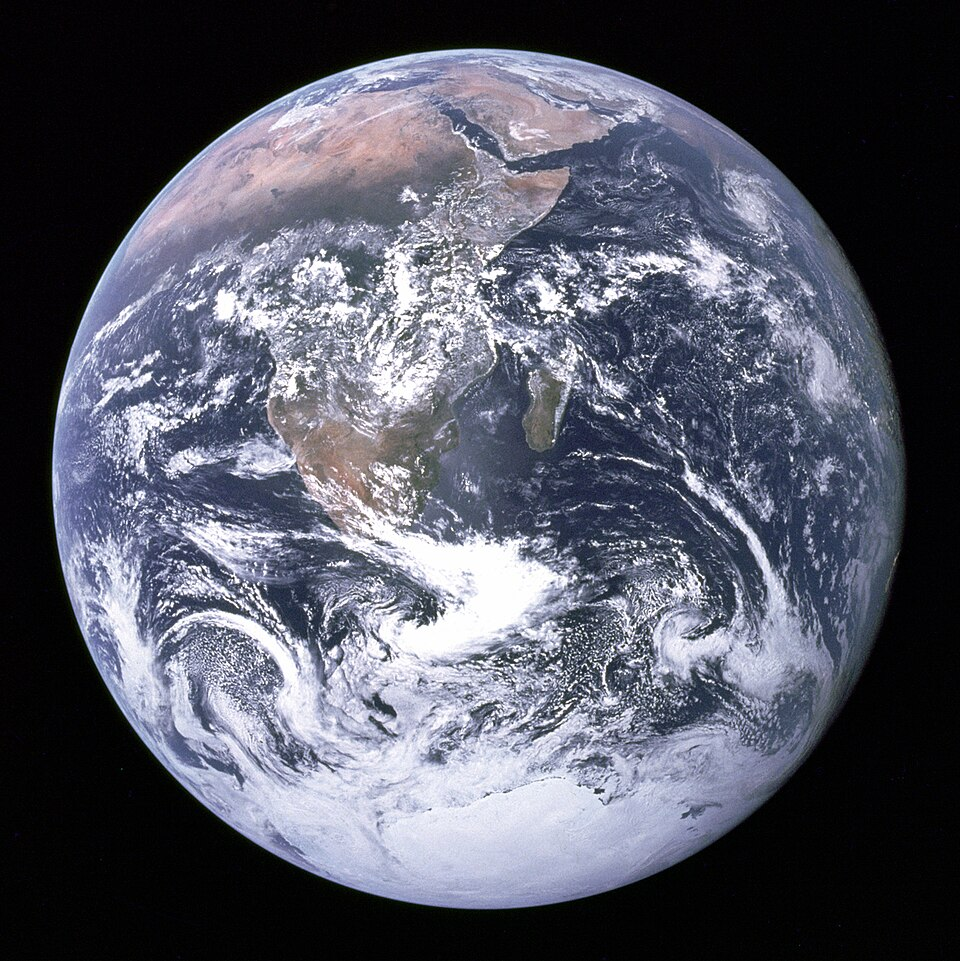
\includegraphics[width=50mm]{blue_marble.jpg}}\\[5mm]
	\subcaptionbox{}{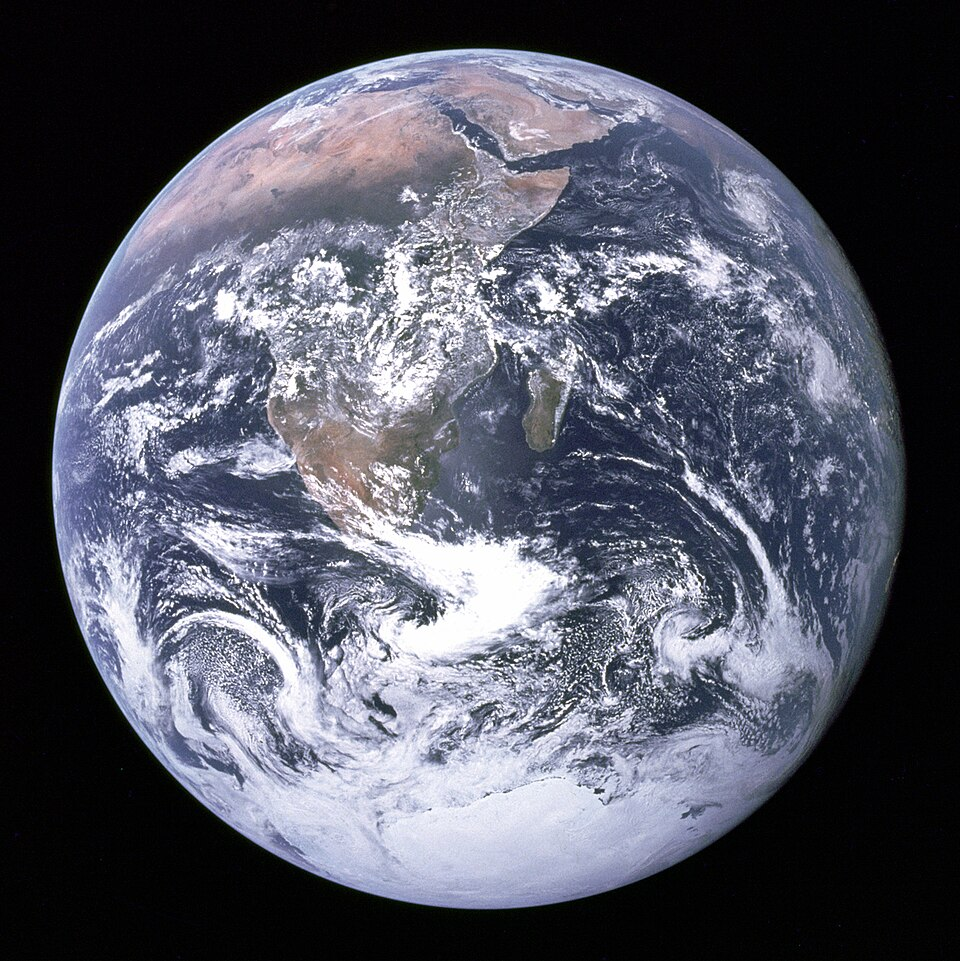
\includegraphics[width=50mm]{blue_marble.jpg}}
	\subcaptionbox{}{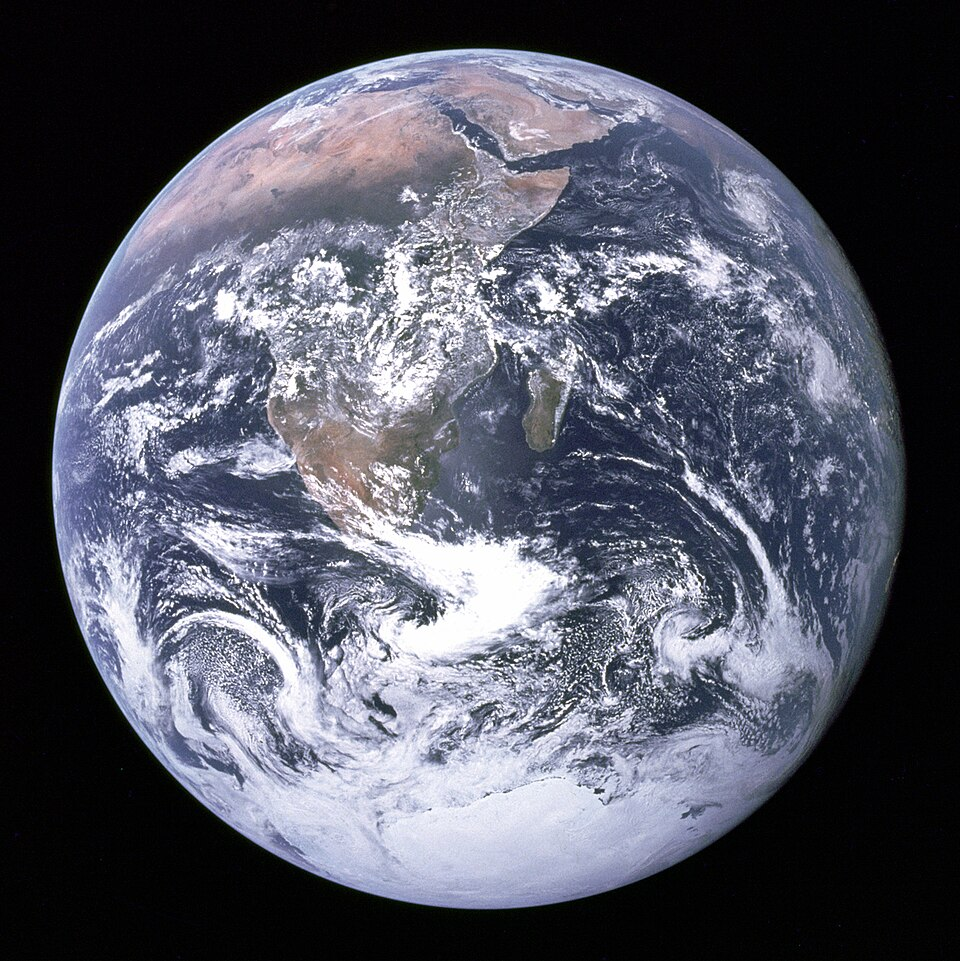
\includegraphics[width=50mm]{blue_marble.jpg}}
	\caption{Multiple subfigures using the \texttt{subcaption} package.}
	\label{fig:subfigures}
\end{figure}


\section{Introduction}
\lipsum[1-2]

\section{Introduction}
\lipsum[1-2]

\section{Introduction}
\lipsum[1-2]

\subsection{Introduction}
\lipsum[1-2]

\section{Introduction}
\lipsum[1-2]

\subsection{Introduction}
\lipsum[1-2]

\printbibliography
\end{document}
